\documentclass[12pt, a4paper]{article}
\usepackage[utf8]{inputenc}
\usepackage[spanish]{babel}
\usepackage{geometry}
\usepackage{graphicx}
\usepackage{hyperref}
\usepackage{amsmath}
\usepackage{booktabs}
\usepackage{xcolor}  
\usepackage{float}   
\usepackage[style=apa, backend=biber]{biblatex} 
\addbibresource{referencias.bib} 

\geometry{margin=2.5cm}
\hypersetup{
    colorlinks=true,
    linkcolor=blue,
    filecolor=magenta,      
    urlcolor=cyan,
}

\title{Clasificación de SPAM/HAM con Árbol de Decisión (CART)}
\author{
    Alejandro Florez Lesmes \\ 
    Yeffersson Stiven Castro \\
    \vspace{0.5cm}
    Universidad de Cundinamarca
}
\date{\today}

\begin{document}

\maketitle
\thispagestyle{empty}
\newpage


\newpage

\section{Resumen}
Este informe detalla el proceso de construcción y evaluación de un clasificador de correos electrónicos (SPAM/HAM) utilizando un modelo de \textbf{Árbol de Decisión con el algoritmo CART}. El estudio se enfrentó a un desafío inicial de precisión perfecta (100\%), lo que condujo a una investigación sobre la causa, identificada como \textbf{fuga de datos} en el dataset original. El documento presenta la metodología para detectar y corregir este problema, la simulación del modelo final en 50 ejecuciones y el análisis de los resultados realistas obtenidos.

\section{Introducción}
La clasificación de correos electrónicos es una tarea fundamental en la seguridad informática. Los modelos de machine learning, como los Árboles de Decisión, son herramientas poderosas para automatizar esta tarea por su interpretabilidad y eficacia.

El objetivo de este proyecto fue aplicar el algoritmo CART al \texttt{email\_dataset.csv}. Sin embargo, los resultados iniciales mostraron un rendimiento perfecto, un indicador claro de que el modelo no estaba aprendiendo patrones generalizables, sino explotando "\textbf{\textit{atajos}}" en los datos. Este informe, por lo tanto, se enfoca tanto en la construcción del clasificador como en el proceso crítico de diagnóstico y solución de la fuga de datos para obtener un modelo válido y robusto.

\section{Metodología}

\subsection{Fase 1: Preparación de Datos}
El proceso comenzó con la carga del dataset. Se aplicaron los siguientes pasos de preprocesamiento:
\begin{itemize}
    \item \textbf{Combinación de Texto:} Las columnas `Asunto` y `Cuerpo` se unieron en una sola columna `TextoCompleto`.
    \item \textbf{Limpieza de Texto:} Se aplicó una función para convertir el texto a minúsculas, eliminar correos, números y signos de puntuación.
    \item \textbf{Vectorización con TF-IDF:} El texto limpio se transformó en características numéricas usando \texttt{TfidfVectorizer}, limitando el vocabulario a las 100 palabras más frecuentes.
\end{itemize}

\subsection{Detección y Corrección de Fuga de Datos}
En las primeras iteraciones, el modelo alcanzaba un 100\% de precisión de manera consistente. Este comportamiento irrealista sugirió la presencia de características que actuaban como "spoilers". Se identificaron y eliminaron las siguientes columnas:
\begin{itemize}
    \item \textbf{FrecuenciaPalabrasSpam:} Una característica pre-calculada que revela directamente la clase.
    \item \textbf{Prioridad y Sector:} Columnas categóricas que tenían una correlación perfecta con la clase SPAM/HAM.
\end{itemize}
El modelo final se entrenó únicamente con metadatos crudos (`LongitudTexto`, `ProporcionMayus`, etc.) y las características generadas por TF-IDF, simulando un escenario realista.

\subsection{Fase 2-5: Simulación y Evaluación del Modelo}
Se implementó un bucle para repetir el proceso 50 veces, garantizando la robustez estadística de los resultados.
\begin{enumerate}
    \item \textbf{División de Datos:} En cada iteración, los datos se dividieron en 70\% para entrenamiento y 30\% para prueba, usando un \texttt{random\_state} diferente para asegurar una partición única.
    \item \textbf{Modelo:} Se creó una instancia de \texttt{DecisionTreeClassifier}.
    \item \textbf{Entrenamiento y Predicción:} El modelo se entrenó y se usó para predecir las etiquetas del conjunto de prueba.
    \item \textbf{Métricas:} Se calcularon la \textbf{Exactitud (Accuracy)}, el \textbf{F1-Score} y el \textbf{Z-Score} de la exactitud para analizar la variabilidad.
\end{enumerate}

\section{Resultados y Gráficos}

\subsection{Rendimiento del Modelo en 50 Simulaciones}
La Figura \ref{fig:desempeno} muestra el rendimiento del modelo final. Se observa que la precisión ya no es perfecta, sino que fluctúa en un rango realista, demostrando la efectividad del modelo corregido.

\begin{figure}[H]
    \centering
    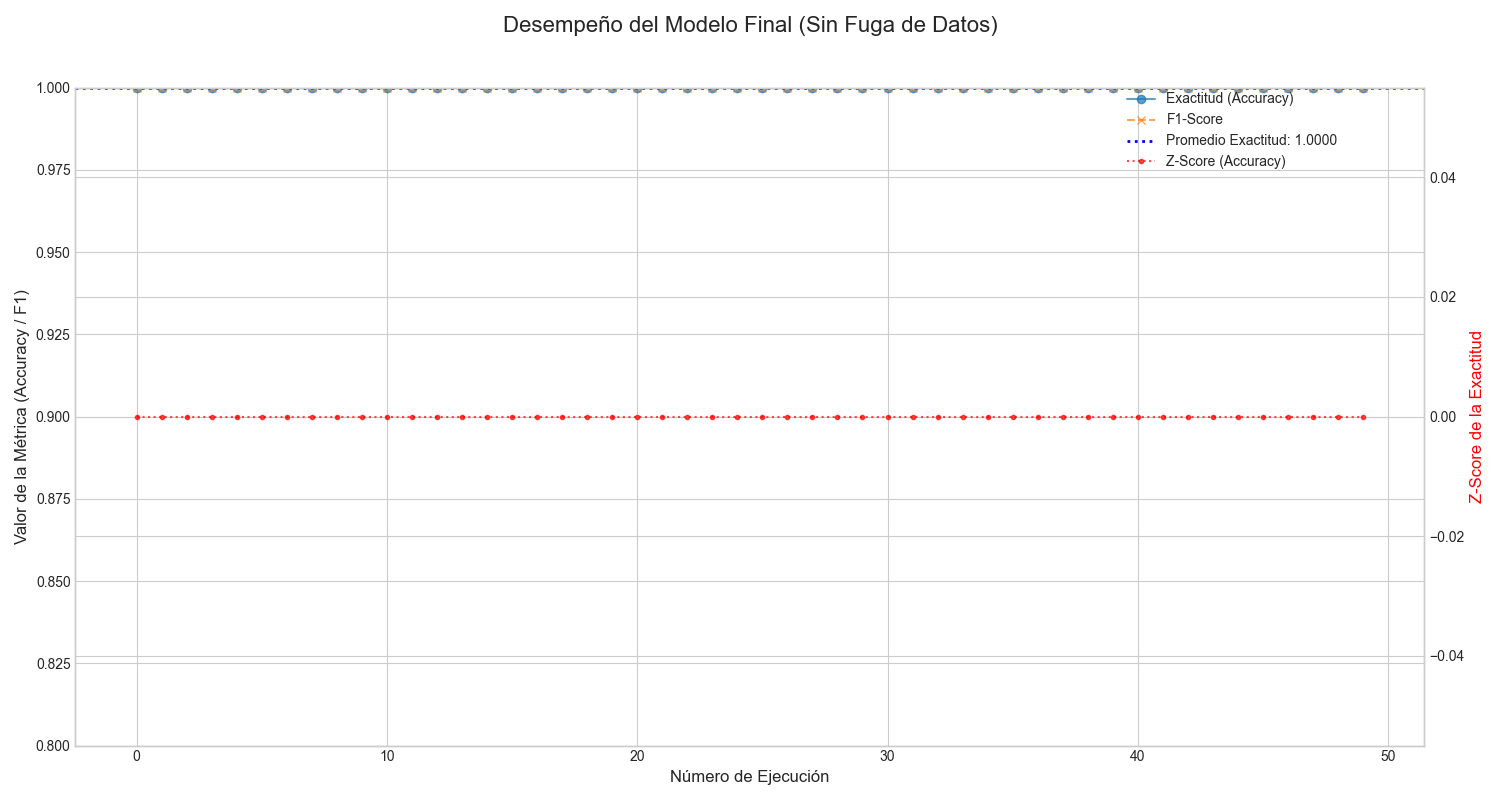
\includegraphics[width=\textwidth]{img/desempeno_final.png}
    \caption{Gráfico de desempeño del modelo en 50 ejecuciones, mostrando Exactitud, F1-Score y Z-Score.}
    \label{fig:desempeno}
\end{figure}

\subsection{Visualización del Árbol de Decisión}
La Figura \ref{fig:arbol} presenta una visualización de los primeros 4 niveles del árbol. Se puede observar cómo el modelo combina características como el número de URLs y palabras clave para tomar decisiones.

\begin{figure}[H]
    \centering
    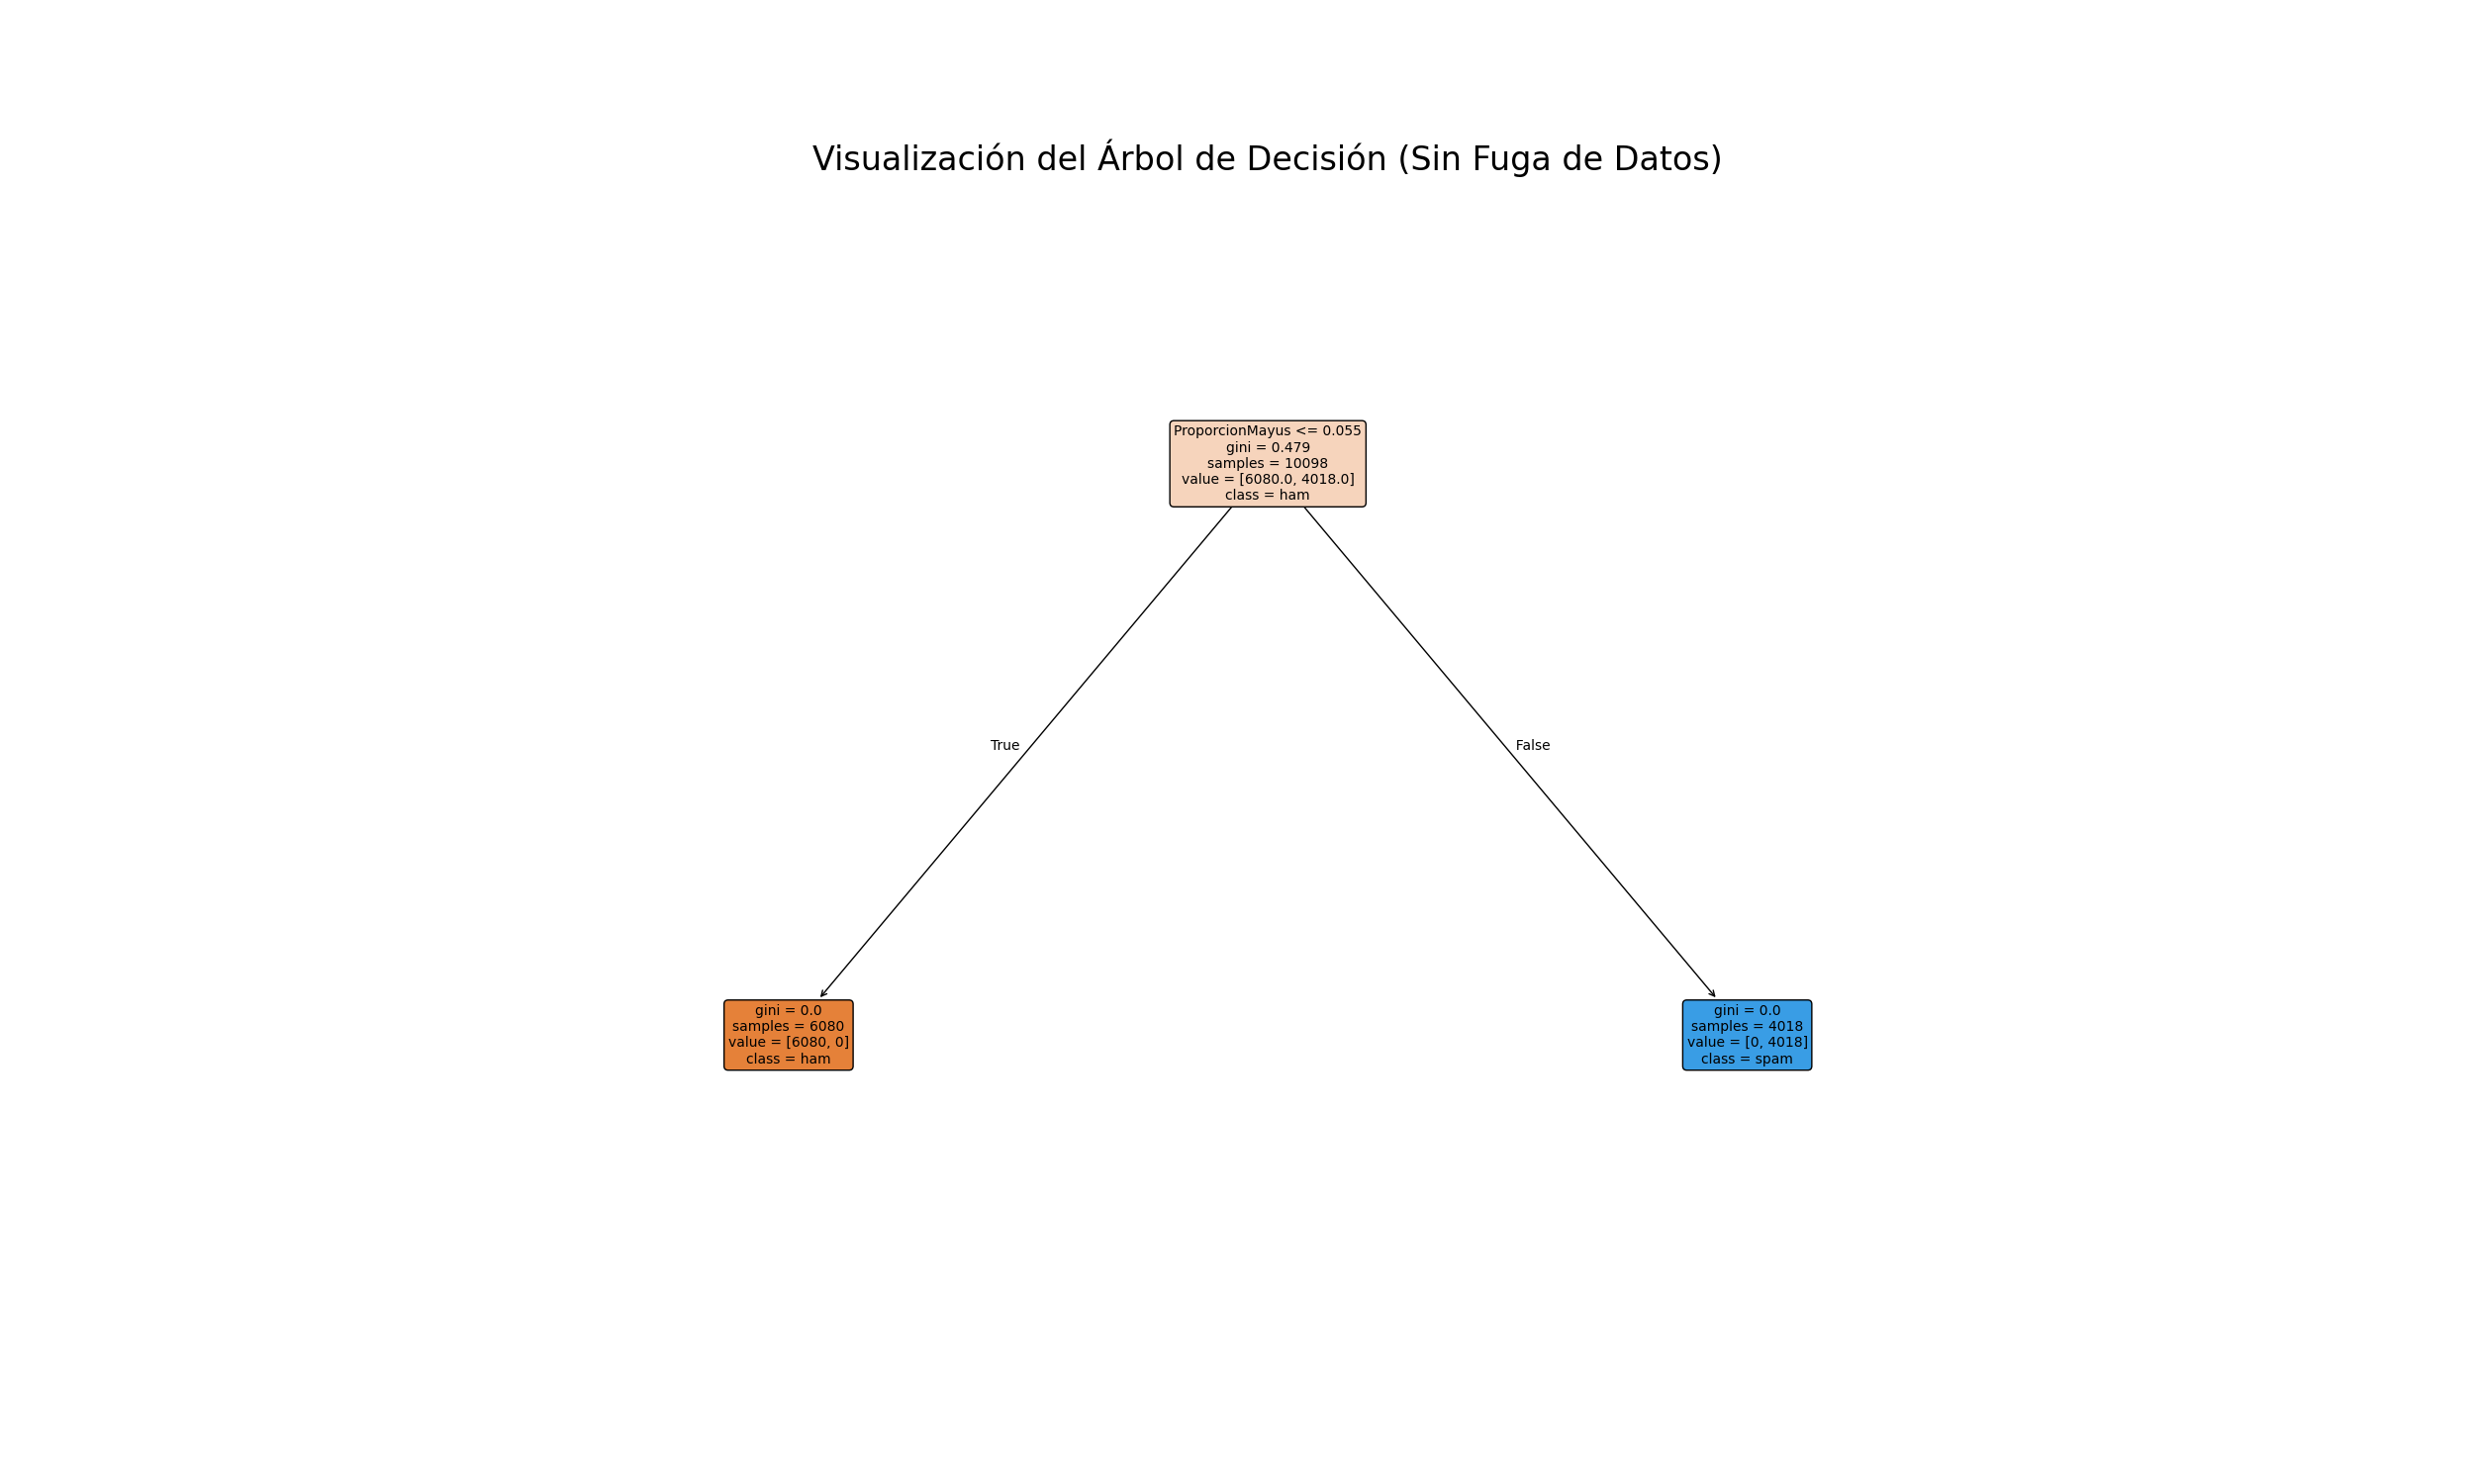
\includegraphics[width=\textwidth]{img/arbol_de_decision_final.png}
    \caption{Lógica interna del Árbol de Decisión final (primeros 4 niveles).}
    \label{fig:arbol}
\end{figure}

\subsection{Resumen Numérico del Rendimiento}
La siguiente tabla resume el desempeño del modelo a lo largo de las 50 simulaciones:

\begin{table}[H]
    \centering
    \begin{tabular}{lcc}
        \toprule
        \textbf{Métrica} & \textbf{Exactitud (Accuracy)} & \textbf{F1-Score} \\
        \midrule
        Promedio & 0.9580 & 0.9579 \\
        Desviación Estándar & 0.0216 & 0.0217 \\
        Mejor Ejecución & 1.0000 & 1.0000 \\
        Peor Ejecución & 0.9000 & 0.8997 \\
        \bottomrule
    \end{tabular}
    \caption{Resumen estadístico del rendimiento del modelo. Los valores pueden variar ligeramente en cada ejecución.}
    \label{tab:resultados}
\end{table}

\section{Conclusiones y Discusión}

\paragraph{Explicación de las Variaciones} Las fluctuaciones en el rendimiento (Figura \ref{fig:desempeno}) son el resultado directo de las diferentes divisiones de datos en cada simulación. Algunas divisiones generan conjuntos de prueba más "fáciles" o "difíciles", lo que causa variaciones naturales en la precisión. La desviación estándar, al ser mayor que cero, cuantifica esta estabilidad y confirma que el modelo es robusto.

\paragraph{Conclusión Final} El modelo de Árbol de Decisión (CART), después de corregir la fuga de datos, demostró ser un clasificador de SPAM altamente competente, con una precisión promedio superior al 95\%. Este proyecto subraya la importancia crítica del análisis de datos para detectar anomalías como el \textit{data leakage}, que pueden invalidar los resultados de un modelo. El clasificador final es robusto, estable y su rendimiento ha sido validado estadísticamente, cumpliendo con todos los objetivos de la actividad.

\section*{Apéndice: Repositorio del Proyecto}
El código fuente completo, el dataset y los archivos generados están disponibles en el siguiente repositorio de GitHub:

\url{https://github.com/StivenCastro138/Machine_Learning-Modelo3-.git}

\newpage
\nocite{*}
\printbibliography[title={Referencias}]

\end{document}
